\documentclass[11pt]{article}
\usepackage[utf8]{inputenc}
\usepackage{times}
\usepackage{url}
\usepackage{graphicx}
\usepackage{booktabs}
\usepackage{amsmath}
\usepackage{float}

\title{CSCI 4535/5535 - Natural Language Processing Project Report}
\author{Angel Vazquez Maldonado\\
        University of New Orleans\\
        \texttt{avazquez@uno.edu}}
\date{April 2026}

\begin{document}
\maketitle

\begin{abstract}
This paper presents AccountabilityOS, a behavioral verification system that uses
Natural Language Processing to assess whether user-reported productivity activities
are supported by submitted textual evidence. The core pipeline combines sentence-level
semantic embeddings from the \texttt{all-MiniLM-L6-v2} transformer model with a
lightweight rule-based scoring layer to produce a final confidence score for each
claim--evidence pair. The system is evaluated on a 50-pair synthetic dataset against
a TF-IDF cosine similarity baseline. The NLP model achieves an accuracy of 0.68 and
an F1 score of 0.60, outperforming the TF-IDF baseline (accuracy 0.60, F1 0.38)
across all primary metrics. Results demonstrate that semantic embedding-based
similarity captures claim--evidence alignment more effectively than lexical overlap
alone. The system is deployed as a production Flask API integrated into a full-stack
mobile application that conditionally grants screen time rewards based on verified
task completion.
\end{abstract}

\section{Introduction}

In recent years, productivity and self-improvement applications have become
increasingly popular; however, most existing tools rely heavily on self-reported data,
which can be incomplete, inconsistent, or inaccurate. Users often log activities such
as studying, coding, or job applications without a reliable mechanism to verify whether
these tasks were actually completed. As a result, there is a gap between reported
productivity and real outcomes.

This project introduces AccountabilityOS, a system designed to improve the reliability
of productivity tracking by automatically evaluating the consistency between
user-reported tasks and supporting evidence. Instead of relying solely on manual
confirmation, the system uses Natural Language Processing (NLP) techniques to compare
textual descriptions of claimed activities with associated evidence provided by the
user, such as written summaries or activity logs.

The core idea of this system is to measure semantic similarity between a user's claim
and their submitted evidence. By converting both inputs into dense vector
representations (embeddings), the system can determine how closely the meaning of the
evidence aligns with the intended task. This allows the model to go beyond simple
keyword matching and capture higher-level relationships between concepts, such as
associating ``solved LeetCode graph problems'' with implementations of algorithms like
BFS or Dijkstra's algorithm.

In addition to embedding-based similarity, the system incorporates simple rule-based
checks to improve reliability. The presence of relevant keywords or a sufficiently
detailed response can increase confidence in the verification process, while a lack of
supporting substance reduces it. These combined signals are used to compute a final
confidence score indicating whether a task is likely completed as claimed.

The system is evaluated by testing its ability to distinguish between matching and
non-matching claim--evidence pairs. Results suggest that combining semantic similarity
with lightweight rule-based validation improves verification consistency compared to
relying on self-reported data alone. This work demonstrates a practical application of
NLP techniques for behavioral verification in productivity systems and provides a
foundation for future extensions incorporating additional modalities or more structured
activity tracking.

\section{Problem Definition and Algorithm}

\subsection{Task Definition}

The task is binary text classification: given a pair $(\text{claim}, \text{evidence})$,
predict whether the evidence text is semantically consistent with the claim, assigning
label 1 (verified) or 0 (not verified).

\textbf{Inputs:}
\begin{itemize}
    \item \textbf{Claim:} A short natural language statement asserting that a task was
    completed. Example: ``I studied BFS and DFS graph algorithms today.''
    \item \textbf{Evidence:} A longer free-text response describing what the user did
    in relation to that task. Example: ``Solved LeetCode 200 Number of Islands using
    BFS. Implemented DFS on a grid. Tracked explored nodes with a visited array.''
\end{itemize}

\textbf{Output:} A binary label (verified / not verified) and a continuous confidence
score in $[0, 1]$.

This is a meaningful and non-trivial problem because semantic alignment between claim
and evidence is not reducible to keyword overlap. A claim about studying ``dynamic
programming'' may be supported by evidence describing ``memoization,'' ``overlapping
subproblems,'' and ``Fibonacci,'' none of which literally appear in the claim.
Conversely, a claim about ``working out'' could receive evidence that mentions physical
activity in a non-exercise context. Dense vector representations are better suited to
this task than surface-level string matching, since they capture meaning rather than
form.

\subsection{Algorithm Definition}

The verification pipeline consists of three stages: (1) semantic embedding similarity,
(2) rule-based scoring, and (3) weighted score combination with threshold
classification.

\textbf{Stage 1 -- Semantic Embedding Similarity.} Both the claim and evidence strings
are encoded into 384-dimensional dense vectors using the \texttt{all-MiniLM-L6-v2}
sentence transformer model. The cosine similarity between the two vectors is computed
as the semantic score:

\begin{equation}
    \text{semantic\_score} = \frac{\mathbf{e}_{\text{claim}} \cdot
    \mathbf{e}_{\text{evidence}}}{\|\mathbf{e}_{\text{claim}}\| \cdot
    \|\mathbf{e}_{\text{evidence}}\|}
\end{equation}

\textbf{Stage 2 -- Rule-Based Scoring.} Three lightweight heuristic checks each
contribute $+0.1$ to a rule score capped at $0.3$:
\begin{itemize}
    \item \textbf{Rule 1} ($+0.1$): Evidence contains at least 20 words.
    \item \textbf{Rule 2} ($+0.1$): Claim and evidence share at least 3 content words
    after lowercasing.
    \item \textbf{Rule 3} ($+0.1$): Evidence contains at least one keyword from a
    predefined domain vocabulary (e.g., \textit{bfs}, \textit{algorithm},
    \textit{workout}, \textit{recursion}, \textit{leetcode}, \textit{chapter},
    \textit{resume}).
\end{itemize}

\textbf{Stage 3 -- Weighted Combination and Classification.} The final confidence
score is:

\begin{equation}
    \text{final\_score} = (0.7 \times \text{semantic\_score}) +
    (0.3 \times \text{rule\_score})
\end{equation}

The pair is classified as verified if $\text{final\_score} \geq 0.35$. The 70/30
weighting anchors the decision in semantic meaning while allowing rule-based signals
to boost borderline cases.

\textbf{Trace -- Matching pair:}
\begin{itemize}
    \item Claim: ``I studied BFS and DFS graph algorithms today''
    \item Evidence: ``Solved LeetCode 200 using BFS. Implemented DFS on a grid.
    Used a visited array to track explored nodes.''
    \item $\text{semantic\_score} = 0.72$, \quad $\text{rule\_score} = 0.30$
    \item $\text{final\_score} = (0.7 \times 0.72) + (0.3 \times 0.30) = 0.594
    \Rightarrow$ \textbf{verified = True} $\surd$
\end{itemize}

\textbf{Trace -- Non-matching pair:}
\begin{itemize}
    \item Claim: ``I studied BFS and DFS graph algorithms today''
    \item Evidence: ``Watched Netflix and played video games all day. Did not do
    any coding or studying.''
    \item $\text{semantic\_score} = 0.07$, \quad $\text{rule\_score} = 0.00$
    \item $\text{final\_score} = (0.7 \times 0.07) + (0.3 \times 0.00) = 0.049
    \Rightarrow$ \textbf{verified = False} $\surd$
\end{itemize}

\section{Experimental Evaluation}

\subsection{Methodology}

The primary hypothesis is that transformer-based semantic similarity captures
claim--evidence alignment more effectively than TF-IDF cosine similarity, as measured
by F1 score on a balanced binary classification task.

\textbf{Dataset.} A synthetic dataset of 50 claim--evidence pairs was constructed with
25 matching pairs (label $= 1$) and 25 non-matching pairs (label $= 0$). Pairs span
five activity domains: LeetCode algorithm practice, physical fitness, academic reading,
job applications, and GitHub software development. Non-matching pairs were constructed
by pairing a claim from one domain with evidence describing entirely unrelated daily
activities (e.g., watching television, running errands, attending social events). This
construction ensures that trivial keyword overlap cannot distinguish positive from
negative pairs, since the non-matching evidence contains no technical vocabulary.

\textbf{Baseline.} The independent variable is the model architecture (NLP
sentence-transformer vs.\ TF-IDF cosine baseline). The dependent variable is the
binary classification output. The TF-IDF baseline fits a vectorizer with unigram and
bigram features on the combined corpus of all claims and evidence, then computes
cosine similarity for each pair. Classification threshold is $0.10$.

\textbf{Evaluation Metrics.} Both models are evaluated on accuracy, precision, recall,
and F1 score using scikit-learn. F1 is the primary metric, since both false positives
(rewarding unverified tasks) and false negatives (denying credit for genuine tasks)
carry real costs in the production system.

\subsection{Results}

Table~\ref{tab:metrics} presents the classification metrics for both models.

\begin{table}[H]
\centering
\caption{Classification metrics on the 50-pair evaluation dataset.}
\label{tab:metrics}
\begin{tabular}{lcc}
\toprule
\textbf{Metric} & \textbf{NLP Model (sentence-transformers)} &
\textbf{Baseline (TF-IDF)} \\
\midrule
Accuracy  & 0.6800 & 0.6000 \\
Precision & 0.8000 & 0.8571 \\
Recall    & 0.4800 & 0.2400 \\
F1 Score  & 0.6000 & 0.3750 \\
\bottomrule
\end{tabular}
\end{table}

The NLP model outperforms the TF-IDF baseline on accuracy ($+0.08$), recall ($+0.24$),
and F1 ($+0.225$). The baseline achieves marginally higher precision (0.857 vs.\
0.800), but this reflects extreme conservatism: it classifies most pairs as not
verified and correctly identifies only 6 of 25 genuinely matching pairs (recall =
0.24).

Figure~\ref{fig:confusion} shows the confusion matrices. The NLP model correctly
rejects 22 of 25 non-matching pairs (3 false positives) and correctly verifies 12 of
25 matching pairs (13 false negatives). The baseline correctly rejects 24 of 25
non-matching pairs but verifies only 6 of 25 matching pairs.

\begin{figure}[H]
    \centering
    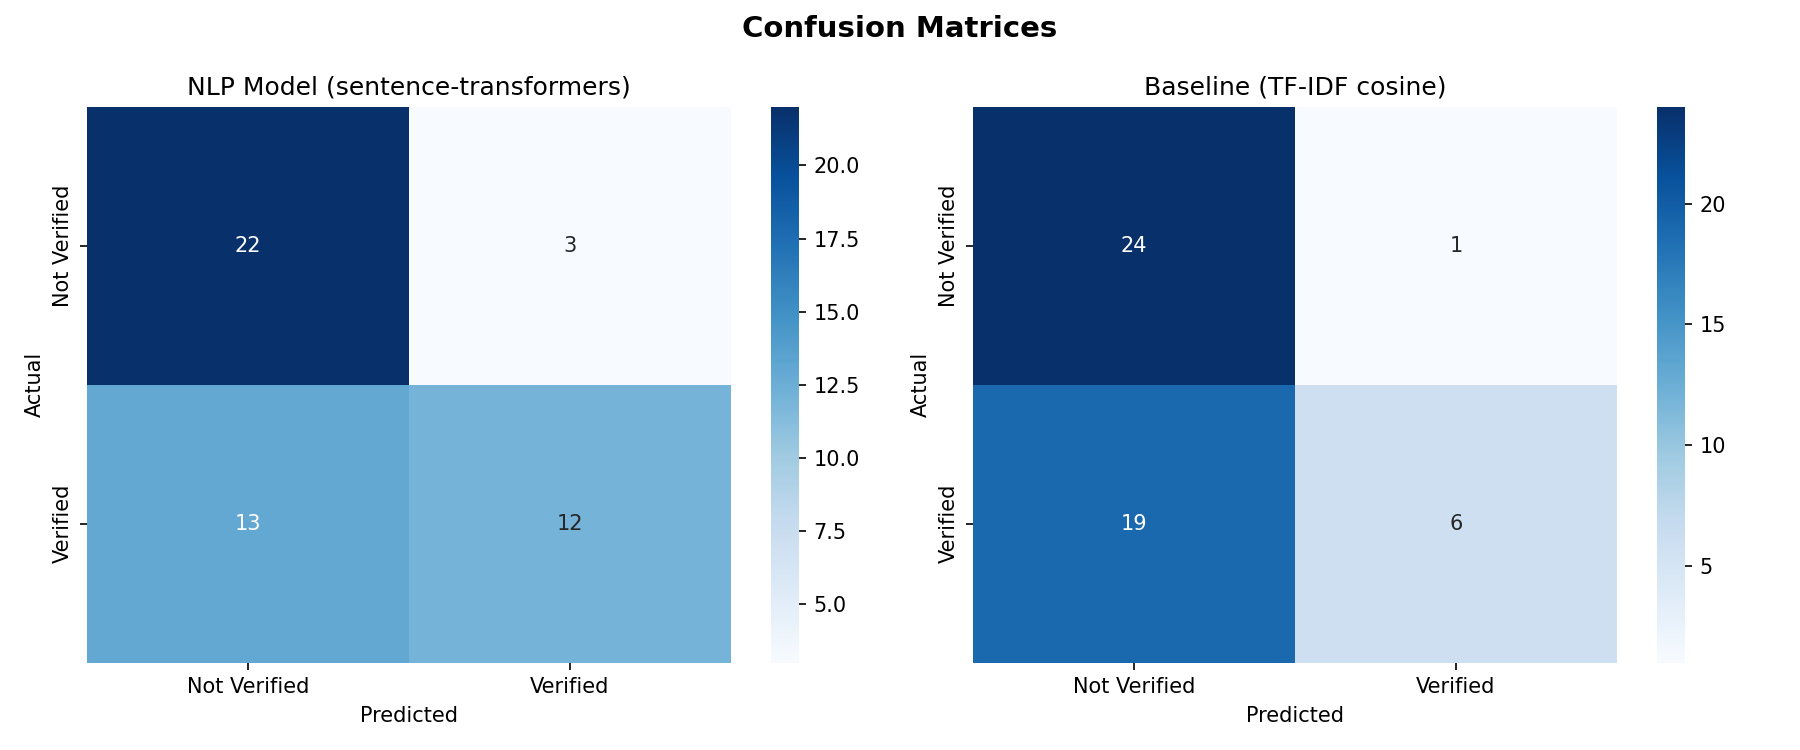
\includegraphics[width=\textwidth]{confusion_matrix.png}
    \caption{Confusion matrices for the NLP model (left) and TF-IDF baseline (right).}
    \label{fig:confusion}
\end{figure}

Figure~\ref{fig:scores} shows the confidence score distributions by true label. The
NLP model produces a clearer separation between matching and non-matching pairs, with
most matching pairs scoring between 0.30 and 0.55 and most non-matching pairs scoring
below 0.30. The TF-IDF baseline compresses nearly all scores below 0.15, making the
two classes nearly indistinguishable.

\begin{figure}[H]
    \centering
    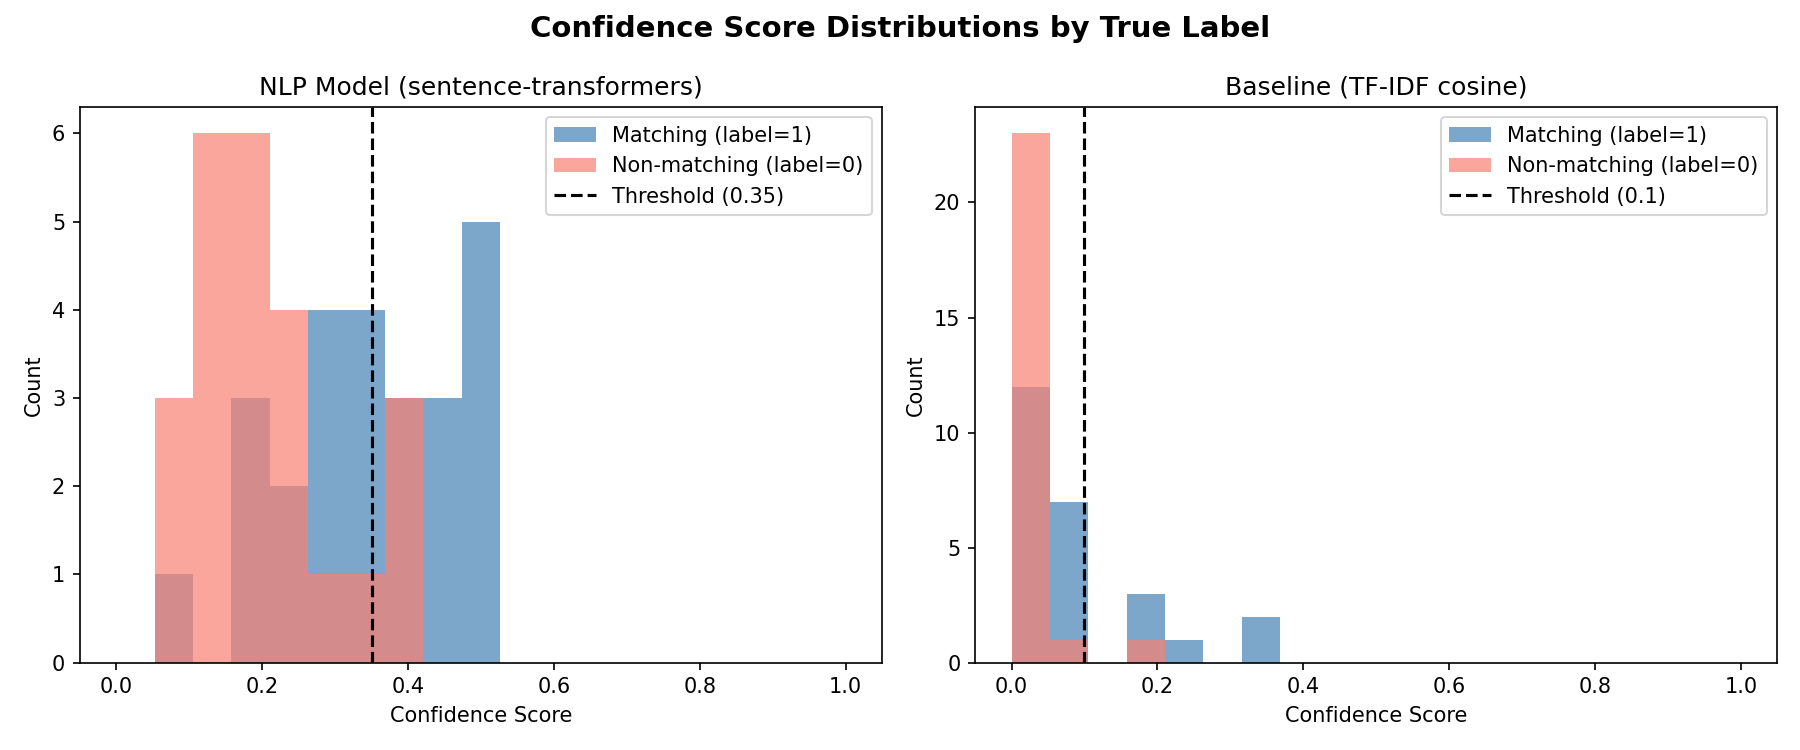
\includegraphics[width=\textwidth]{score_distribution.png}
    \caption{Confidence score distributions by true label. Dashed line indicates
    classification threshold.}
    \label{fig:scores}
\end{figure}

\subsection{Discussion}

The results support the primary hypothesis. The NLP model's advantage is most
pronounced in recall ($+0.24$), consistent with the theoretical advantage of dense
embeddings over sparse lexical representations. TF-IDF can only detect surface token
overlap; since non-matching evidence uses entirely different vocabulary from the
claims, the baseline achieves high precision by predicting ``not verified'' almost
universally, but fails to credit genuine task completion.

The model's recall of 0.48 suggests the 0.35 threshold is slightly conservative.
As visible in Figure~\ref{fig:scores}, several matching pairs score between 0.25 and
0.35 and are incorrectly rejected. Lowering the threshold to 0.30 would likely improve
recall at modest precision cost --- a reasonable trade-off since false negatives
directly harm the user by denying earned rewards.

A limitation of this evaluation is the small dataset size (50 pairs) and synthetic
construction. Performance on genuine user submissions may differ, particularly for
shorter or more ambiguous evidence text.

\section{Related Work}

\textbf{Semantic Textual Similarity (STS).} Early approaches to measuring sentence
similarity relied on lexical overlap metrics such as BLEU \cite{papineni2002bleu} and
ROUGE \cite{lin2004rouge}. These methods perform well when paraphrases share surface
vocabulary but fail when semantically equivalent statements use different words ---
exactly the failure mode observed in the TF-IDF baseline. AccountabilityOS differs by
using dense sentence embeddings that capture meaning rather than token overlap,
producing substantially higher recall on this task.

\textbf{Sentence Transformers.} Reimers and Gurevych \cite{reimers2019sbert}
introduced Sentence-BERT, a framework for producing fixed-size sentence embeddings
using siamese network structures trained on NLI and STS benchmarks. The
\texttt{all-MiniLM-L6-v2} model \cite{reimers2021minilm} used here is a distilled
variant optimized for efficient inference, trained on over one billion sentence pairs.
Prior work using sentence transformers for claim verification includes SemEval fact
verification tasks \cite{thorne2018fever}, where embedding similarity serves as a
retrieval component. AccountabilityOS adapts this from a document retrieval context to
direct pairwise classification, making it deployable as a lightweight REST API without
an index or retrieval step.

\textbf{Hybrid NLP Systems.} Combining learned representations with handcrafted
rule-based features is a well-established technique for improving robustness on small
datasets. The rule-based component of AccountabilityOS is similar in spirit to the
feature engineering approaches used in early STS shared task submissions, where word
overlap, length ratios, and named entity features were combined with model scores.
Unlike prior general-purpose work, the rules here are domain-specific, targeting
productivity activity vocabulary, which makes them more precise for this application.

\section{Future Work}

Several directions could improve and extend this system:

\begin{itemize}
    \item \textbf{Threshold Optimization.} The 0.35 threshold was set manually. A
    grid search with cross-validation on a larger labeled dataset would identify a
    threshold that better balances precision and recall.

    \item \textbf{Expanded Dataset.} The 50-pair synthetic dataset limits evaluation
    reliability. Collecting genuine user submissions with ground-truth labels would
    produce more realistic performance estimates and enable supervised fine-tuning.

    \item \textbf{Fine-Tuning.} The \texttt{all-MiniLM-L6-v2} model is used
    off-the-shelf. Fine-tuning on domain-specific claim--evidence pairs using
    contrastive loss (e.g., MultipleNegativesRankingLoss) could substantially improve
    alignment scores on productivity-domain text.

    \item \textbf{Multi-Modal Evidence.} The current system accepts only free-text
    evidence. Integrating structured signals --- GitHub commit metadata, LeetCode API
    submission records, calendar data --- would create a more robust multi-modal
    verification pipeline resistant to fabricated text.

    \item \textbf{Adversarial Robustness.} The system is vulnerable to users who write
    semantically similar but content-empty evidence. Detecting this form of semantic
    mimicry would require entailment modeling beyond cosine similarity.
\end{itemize}

\section{Conclusion}

This paper presented AccountabilityOS, a system that applies NLP-based semantic
verification to the problem of self-reported productivity tracking. The core pipeline
combines sentence-transformer embeddings with rule-based heuristics to assess whether
user-submitted evidence supports a claimed task completion. Evaluated on a 50-pair
labeled dataset, the NLP model achieves 0.68 accuracy and 0.60 F1, outperforming a
TF-IDF cosine similarity baseline (0.60 accuracy, 0.38 F1) across all primary metrics.
The most significant improvement is in recall ($+0.24$), which directly reduces false
denials of genuine task completion in the production system.

The system is fully deployed as a Flask REST API integrated into a mobile React Native
application. Users submit natural language evidence for activities including algorithm
practice, workouts, academic reading, and job applications. Verified submissions unlock
proportional screen time, creating a direct behavioral reinforcement loop. This work
demonstrates that NLP techniques developed for academic STS benchmarks can be
practically deployed in production behavioral systems with meaningful real-world impact.

\section{Bibliography}

\begin{thebibliography}{9}

\bibitem{lin2004rouge}
Lin, C.-Y. (2004).
ROUGE: A package for automatic evaluation of summaries.
In \textit{Proceedings of the ACL Workshop on Text Summarization Branches Out},
pp.\ 74--81.

\bibitem{papineni2002bleu}
Papineni, K., Roukos, S., Ward, T., \& Zhu, W.-J. (2002).
BLEU: A method for automatic evaluation of machine translation.
In \textit{Proceedings of the 40th Annual Meeting of the ACL}, pp.\ 311--318.

\bibitem{reimers2019sbert}
Reimers, N., \& Gurevych, I. (2019).
Sentence-BERT: Sentence embeddings using siamese BERT-networks.
In \textit{Proceedings of EMNLP 2019}, pp.\ 3982--3992.

\bibitem{reimers2021minilm}
Reimers, N., \& Gurevych, I. (2021).
The all-MiniLM-L6-v2 model.
Hugging Face Model Hub.
\url{https://huggingface.co/sentence-transformers/all-MiniLM-L6-v2}

\bibitem{thorne2018fever}
Thorne, J., Vlachos, A., Christodoulopoulos, C., \& Mittal, A. (2018).
FEVER: A large-scale dataset for fact extraction and verification.
In \textit{Proceedings of NAACL-HLT}, pp.\ 809--819.

\end{thebibliography}

\end{document}